%!TEX root = ../thesis.tex
\chapter{Results and discussion}
\label{chapter:results}

In order to test the robustness of the numerical integration routine, we checked that the results agreed with the FRW bending angle \autoref{eq:series-expansion-R} to at least within $0.1\%$. We were also able to reproduce the results presented in \citet{schucker2009strong} to the stated precision. 

A graph of results when we keep the lensing mass $M$ constant and vary $\Omega_{\Lambda}$ can be seen in \autoref{fig:flat-const-m}. On the $y$-axis, we plot the deviation of $D_{S}/D_{LS}$ as a fraction of the standard FRW lensing case (found by substituting \autoref{eq:series-expansion-R} into the lens equation \ref{eq:lens-eqn}), in order to put them on the same scale. We plot the fractional deviation of $D_{S}/D_{LS}$ instead of $D_S$ or $D_{LS}$ alone since they both depend on the numerical result. That is, if we define $s = D_{S}/D_{LS}$ then we are plotting the quantity $s_{\text{numerical}} / s_{\text{FRW}} - 1$. 

\begin{figure}
  \centering
  % 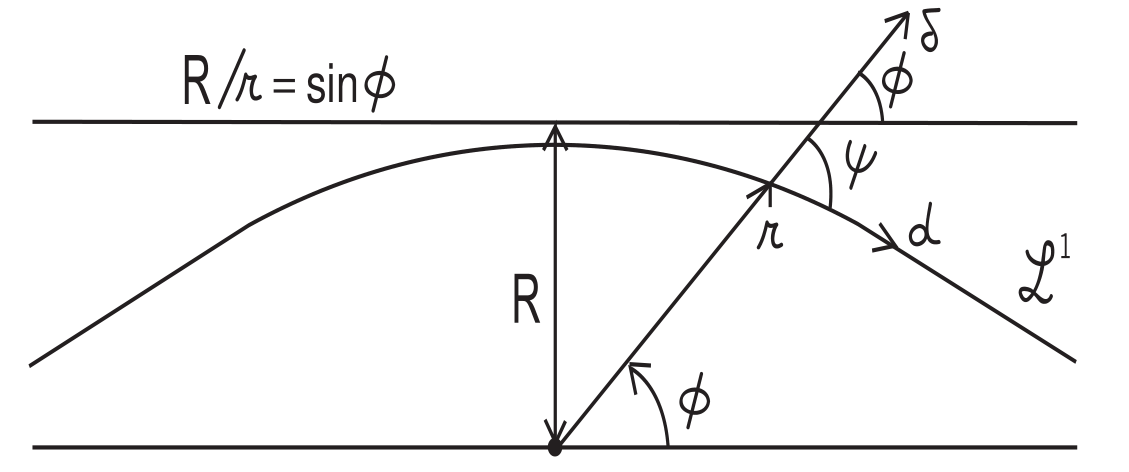
\includegraphics[height=0.5\linewidth]{img/rindler-ishak-2.png}
  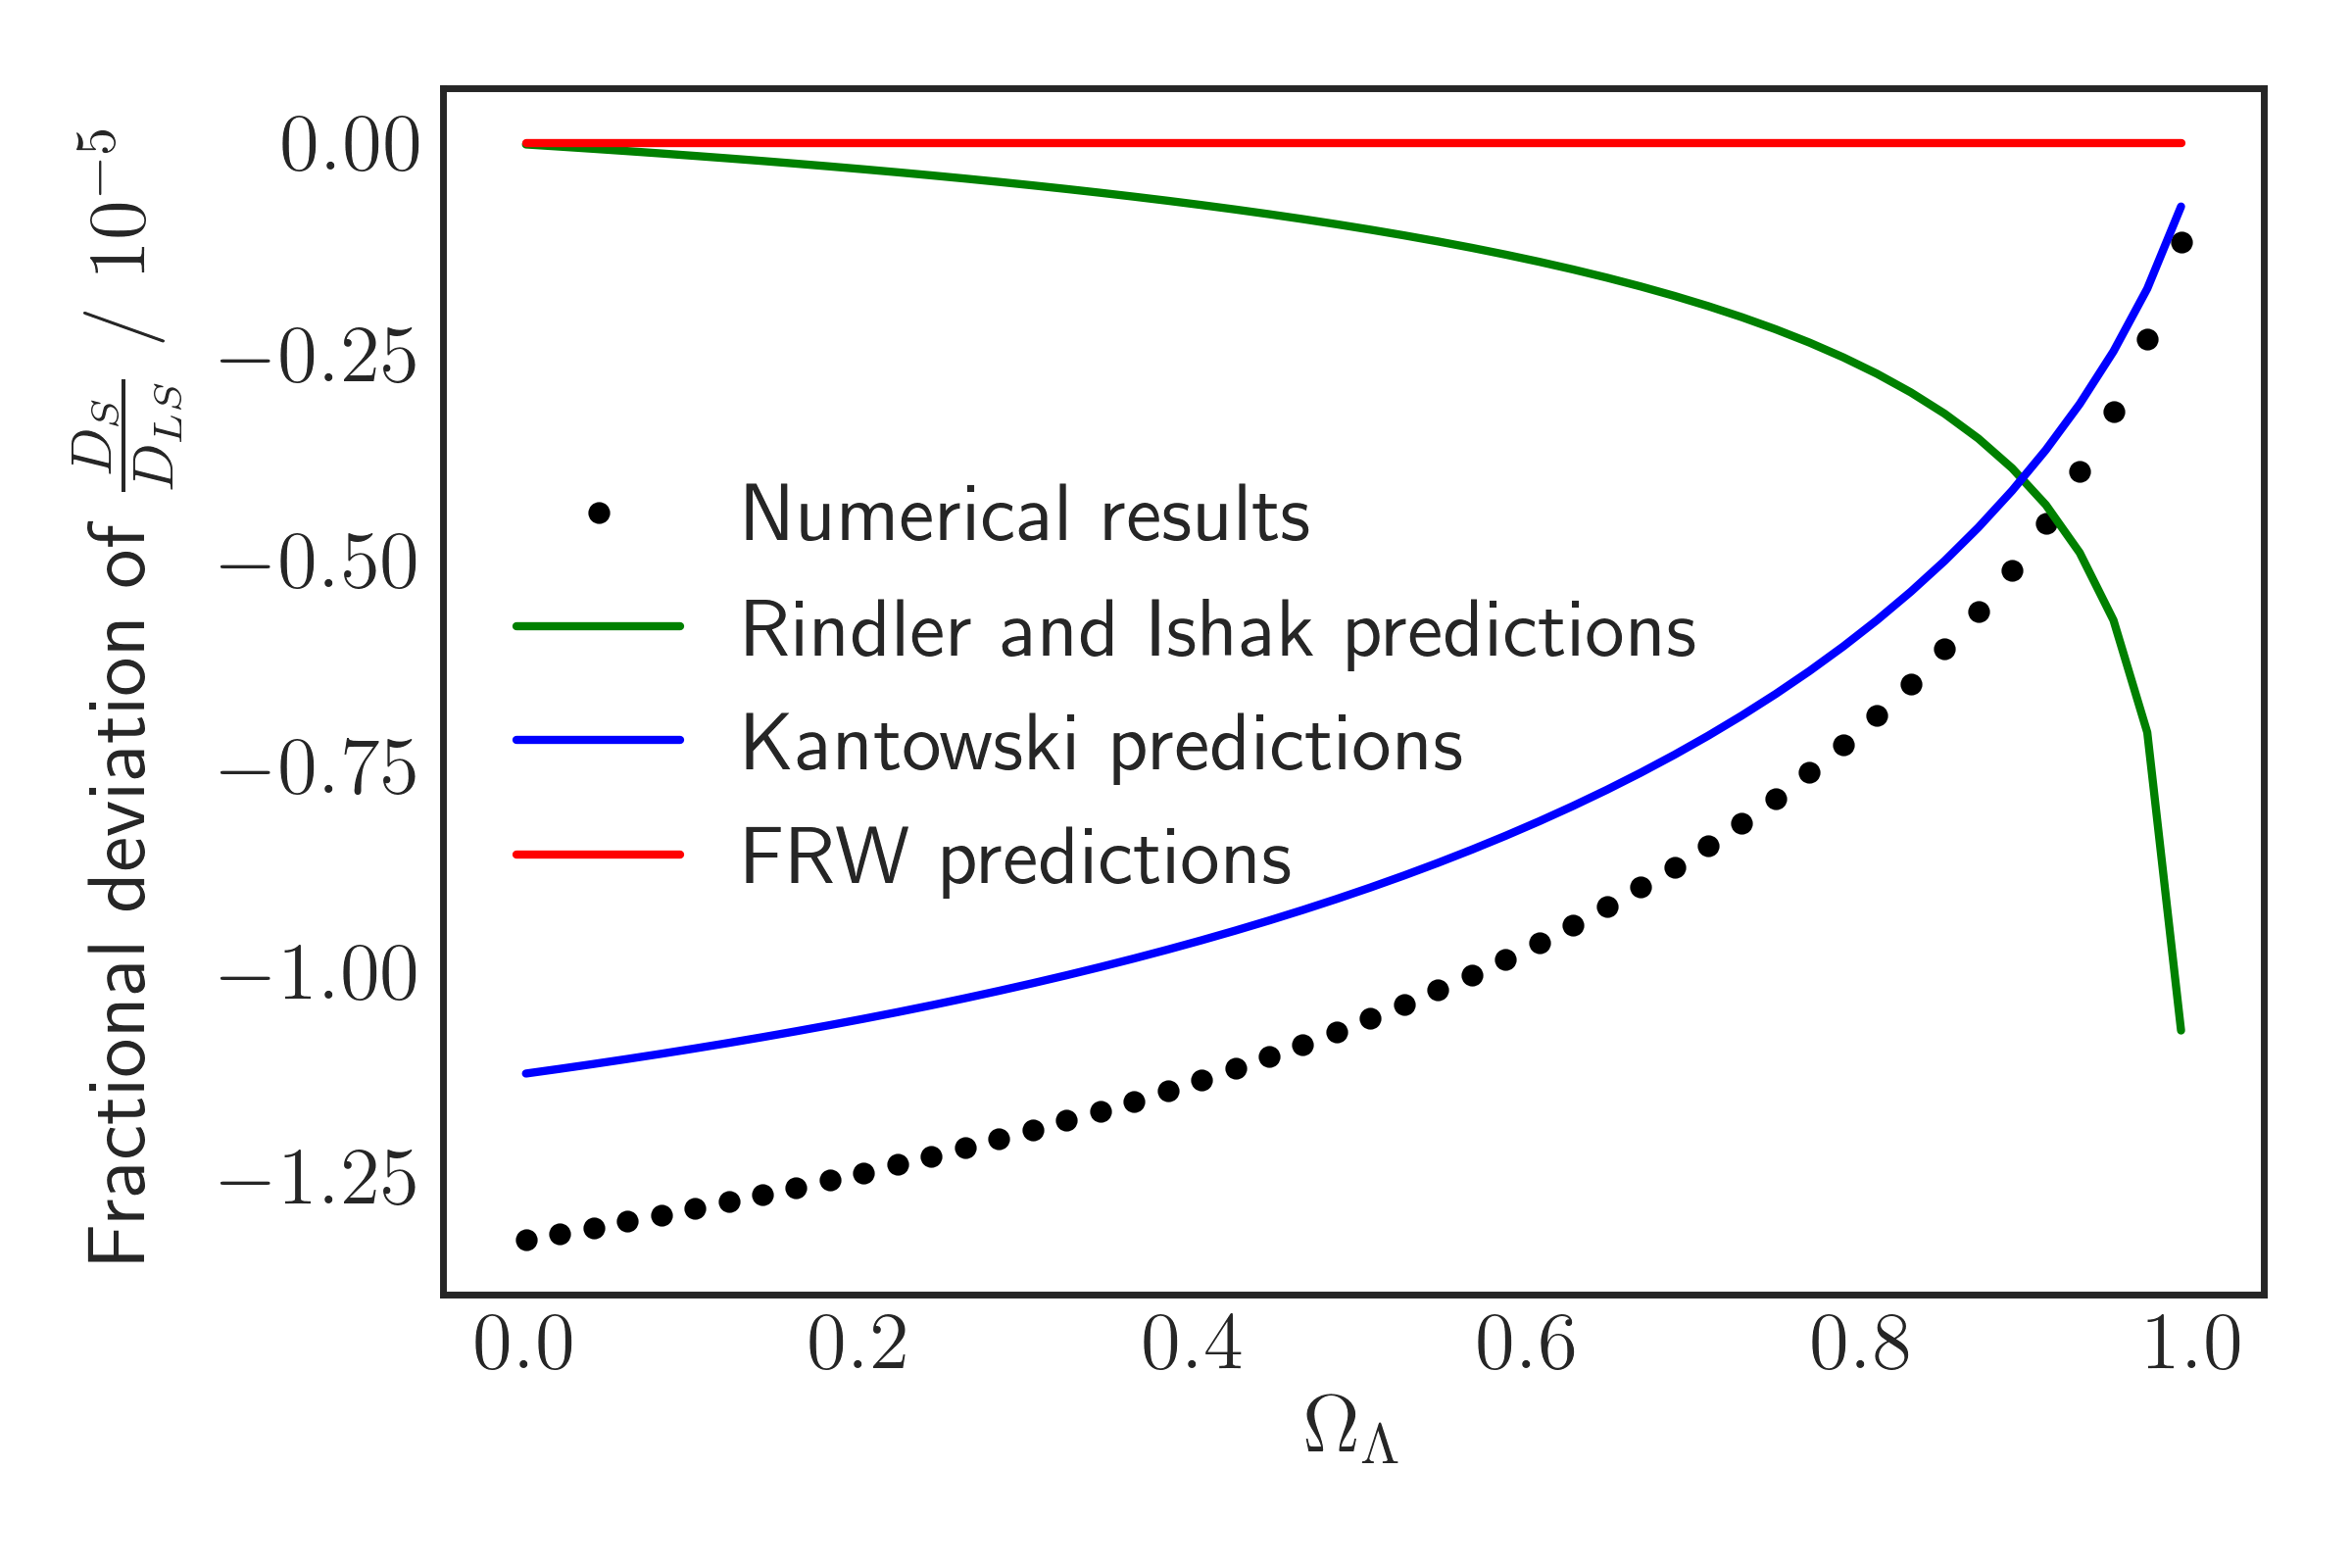
\includegraphics[height=0.5\linewidth]{images/flat.png}
  \caption{These are the results when we keep the mass constant and vary $\Lambda$. The fractional deviations from the expected result in FRW are plotted (\autoref{eq:series-expansion-R} and \autoref{eq:lens-eqn}). The green curve is the Rindler \& Ishak predictions while the blue curve is Kantowski's prediction. Black points are our numerical results. The starting conditions for this are $z_{\text{lens}} = 0.5$ and $\theta_E = 1^{\prime\prime}$, with $\Omega_{\Lambda}$ varying between $0$ and $0.99$. We use $M = 10^{13}M_{\odot}$ and $H_0 = \SI{70}{\kilo\meter\per\second\per\mega\parsec}$.}
  \label{fig:flat-const-m}
\end{figure}

Numerical errors are estimated by varying the tolerance of the integrator. For a certain tolerance level, we group the results obtained from the vicinity of tolerance levels together and find the variance in the numerical result in that range to get a crude estimation of the numerical error. \autoref{fig:errors} shows how the raw $r_{LS}$ coordinate obtained from the integration varies with the relative tolerance level. As is expected, the precision increases as the tolerance level is reduced. For a relative tolerance of $2 \times 10^{-14}$, a conservative estimate obtained by grouping results between $r_{\text{tol}} = 2 \times 10^{-14}$ and $2 \times 10^{-13}$ yields a fractional error of $10^{-8}$. 

\begin{figure}
  \centering
  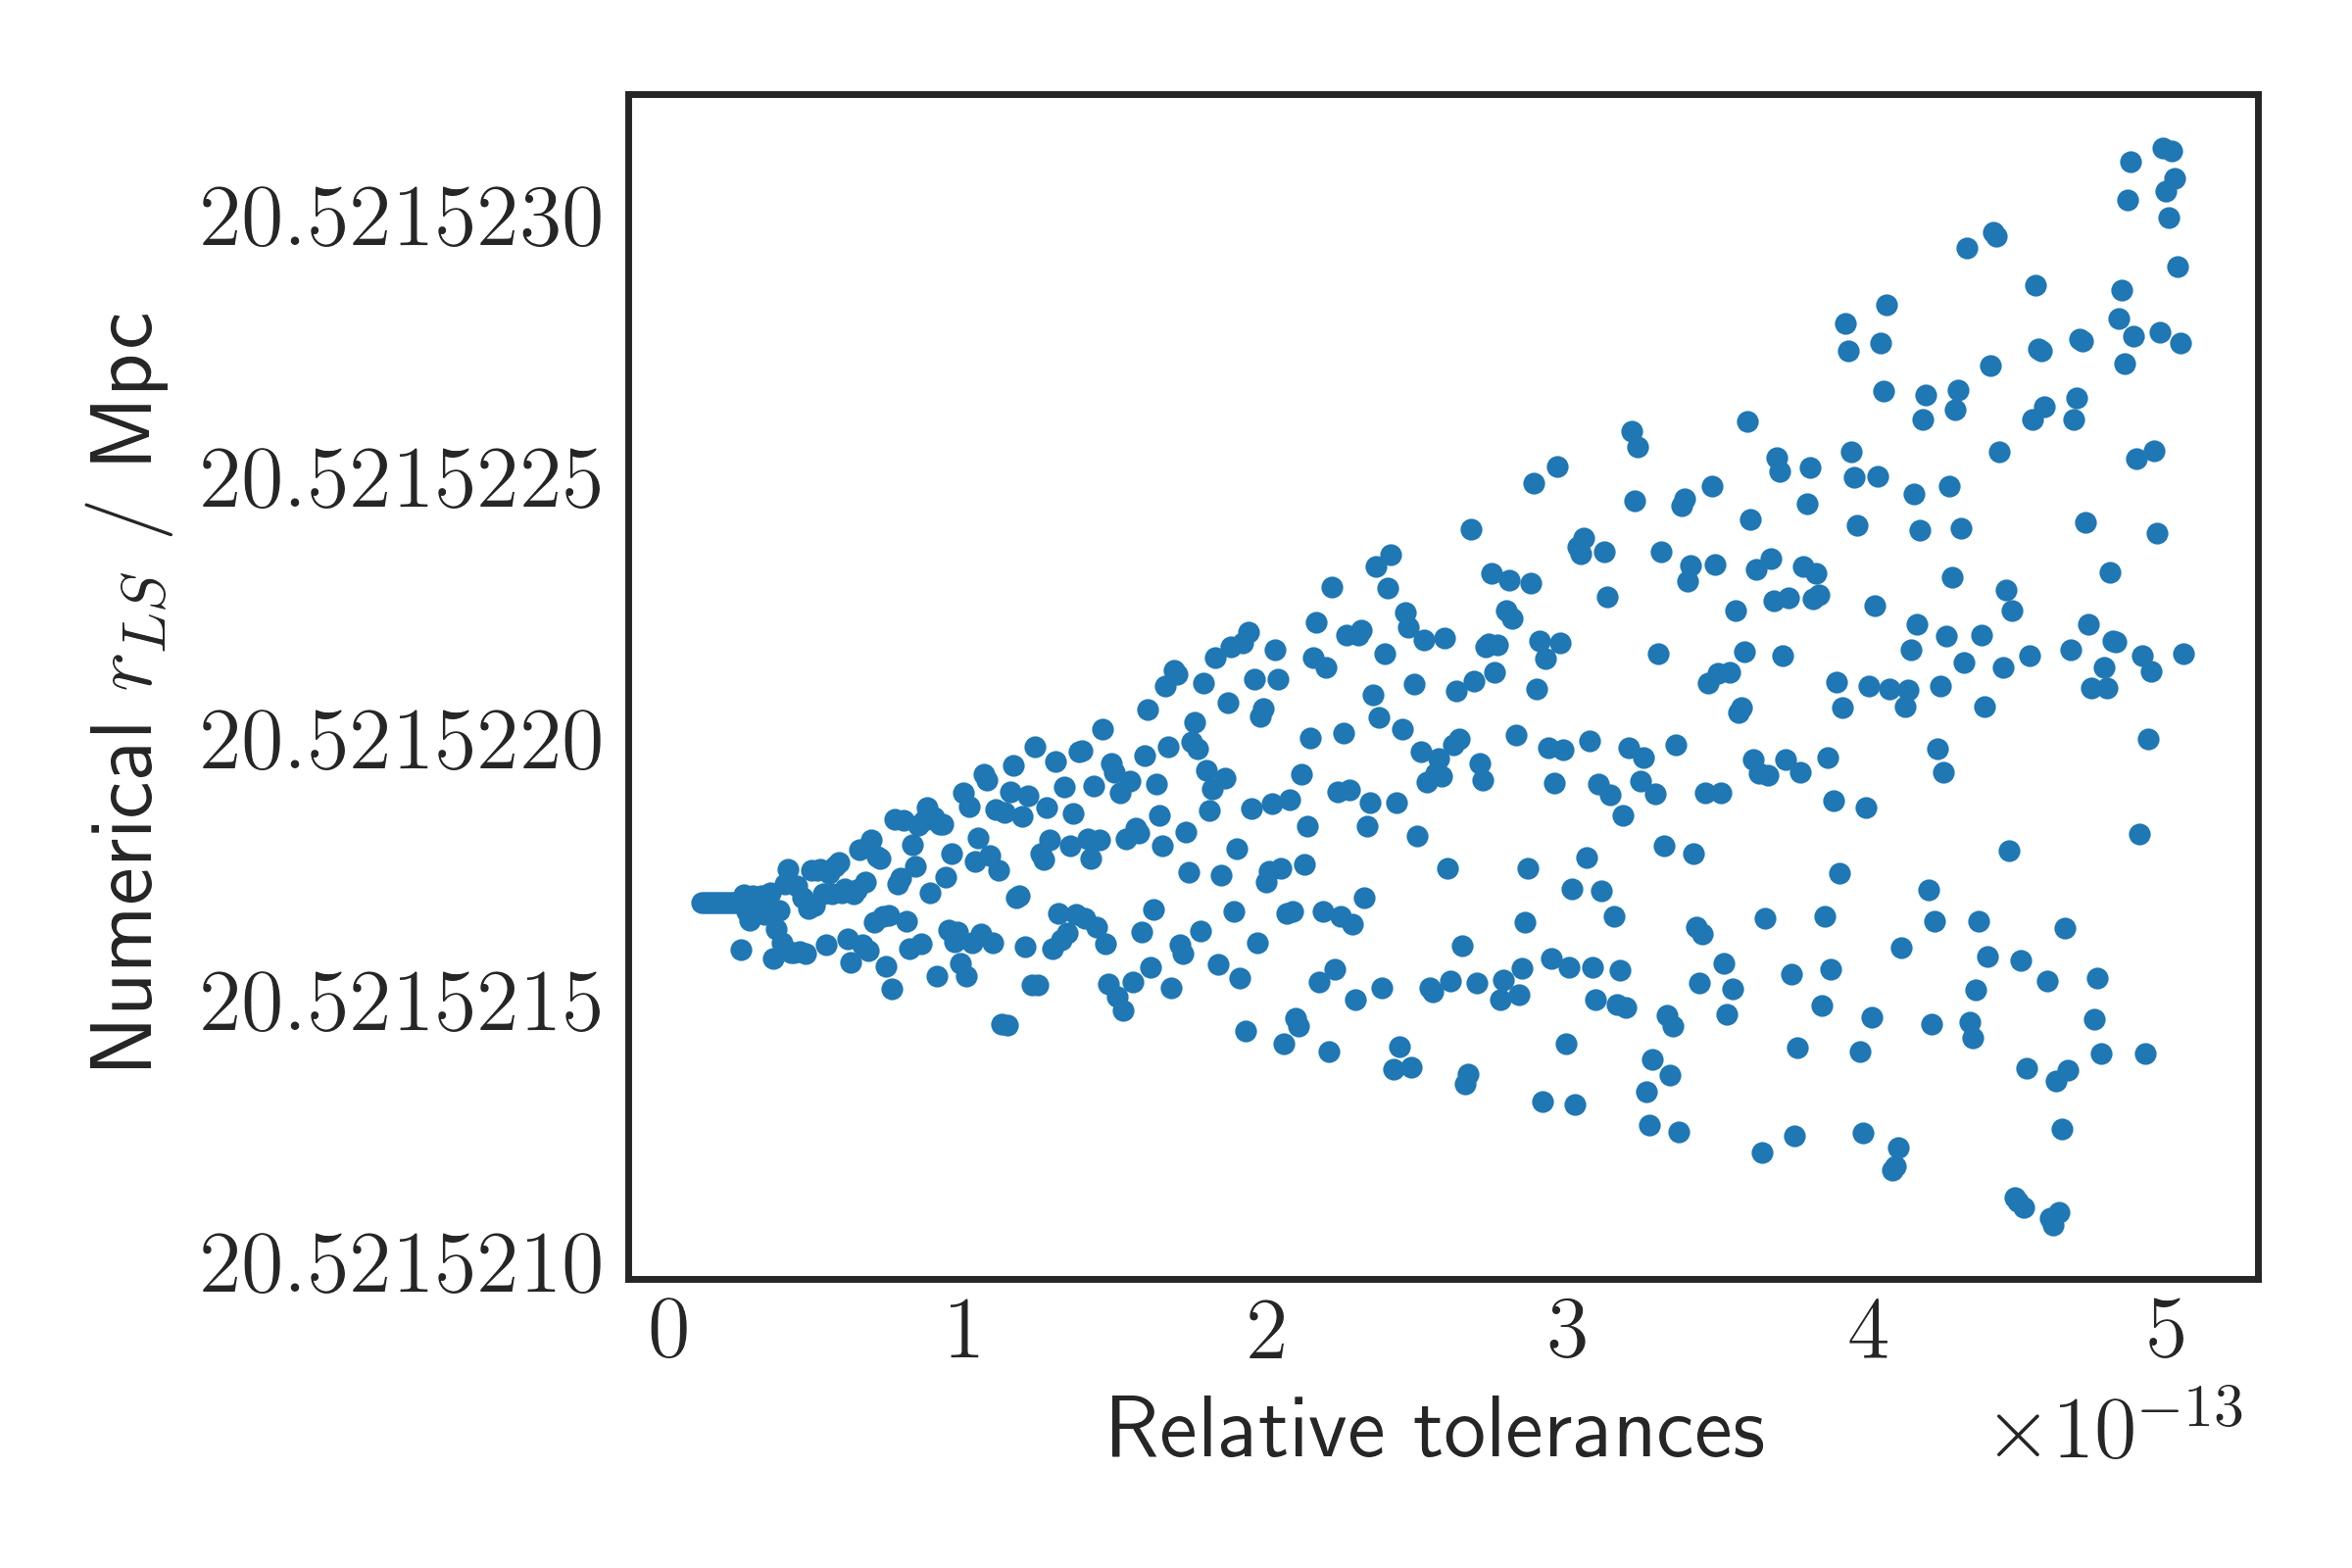
\includegraphics[height=0.5\linewidth]{images/errors.png}
  \caption{Plot of how the numerical result $r_{LS}$ varies with the relative tolerance for $\Omega_{\Lambda} = 0$. }
  \label{fig:errors}
\end{figure}

Our results follow the trend of Kantowski's predictions most closely, with a gap that reduces towards higher $\Lambda$. A possible explanation of this gap can be found by examining the neglected higher order term in Kantowski's predicted bending angle, $\mathcal{O}\left ( 2M/r_0 + \Lambda r_0^2 \right )^{5/2}$. When $\Lambda = 0$, the ratio of this term to his leading order $(4M/r_0^2) \cos^3 \tilde{\phi_1}$ term is of the same order of magnitude as the fractional deviation of our numerical results from Kantowski's predictions. As is expected, our results deviate less from Kantowski's as this ratio decreases, as shown in \autoref{fig:flat-const-m-neglected}. 

\begin{figure}
  \centering
  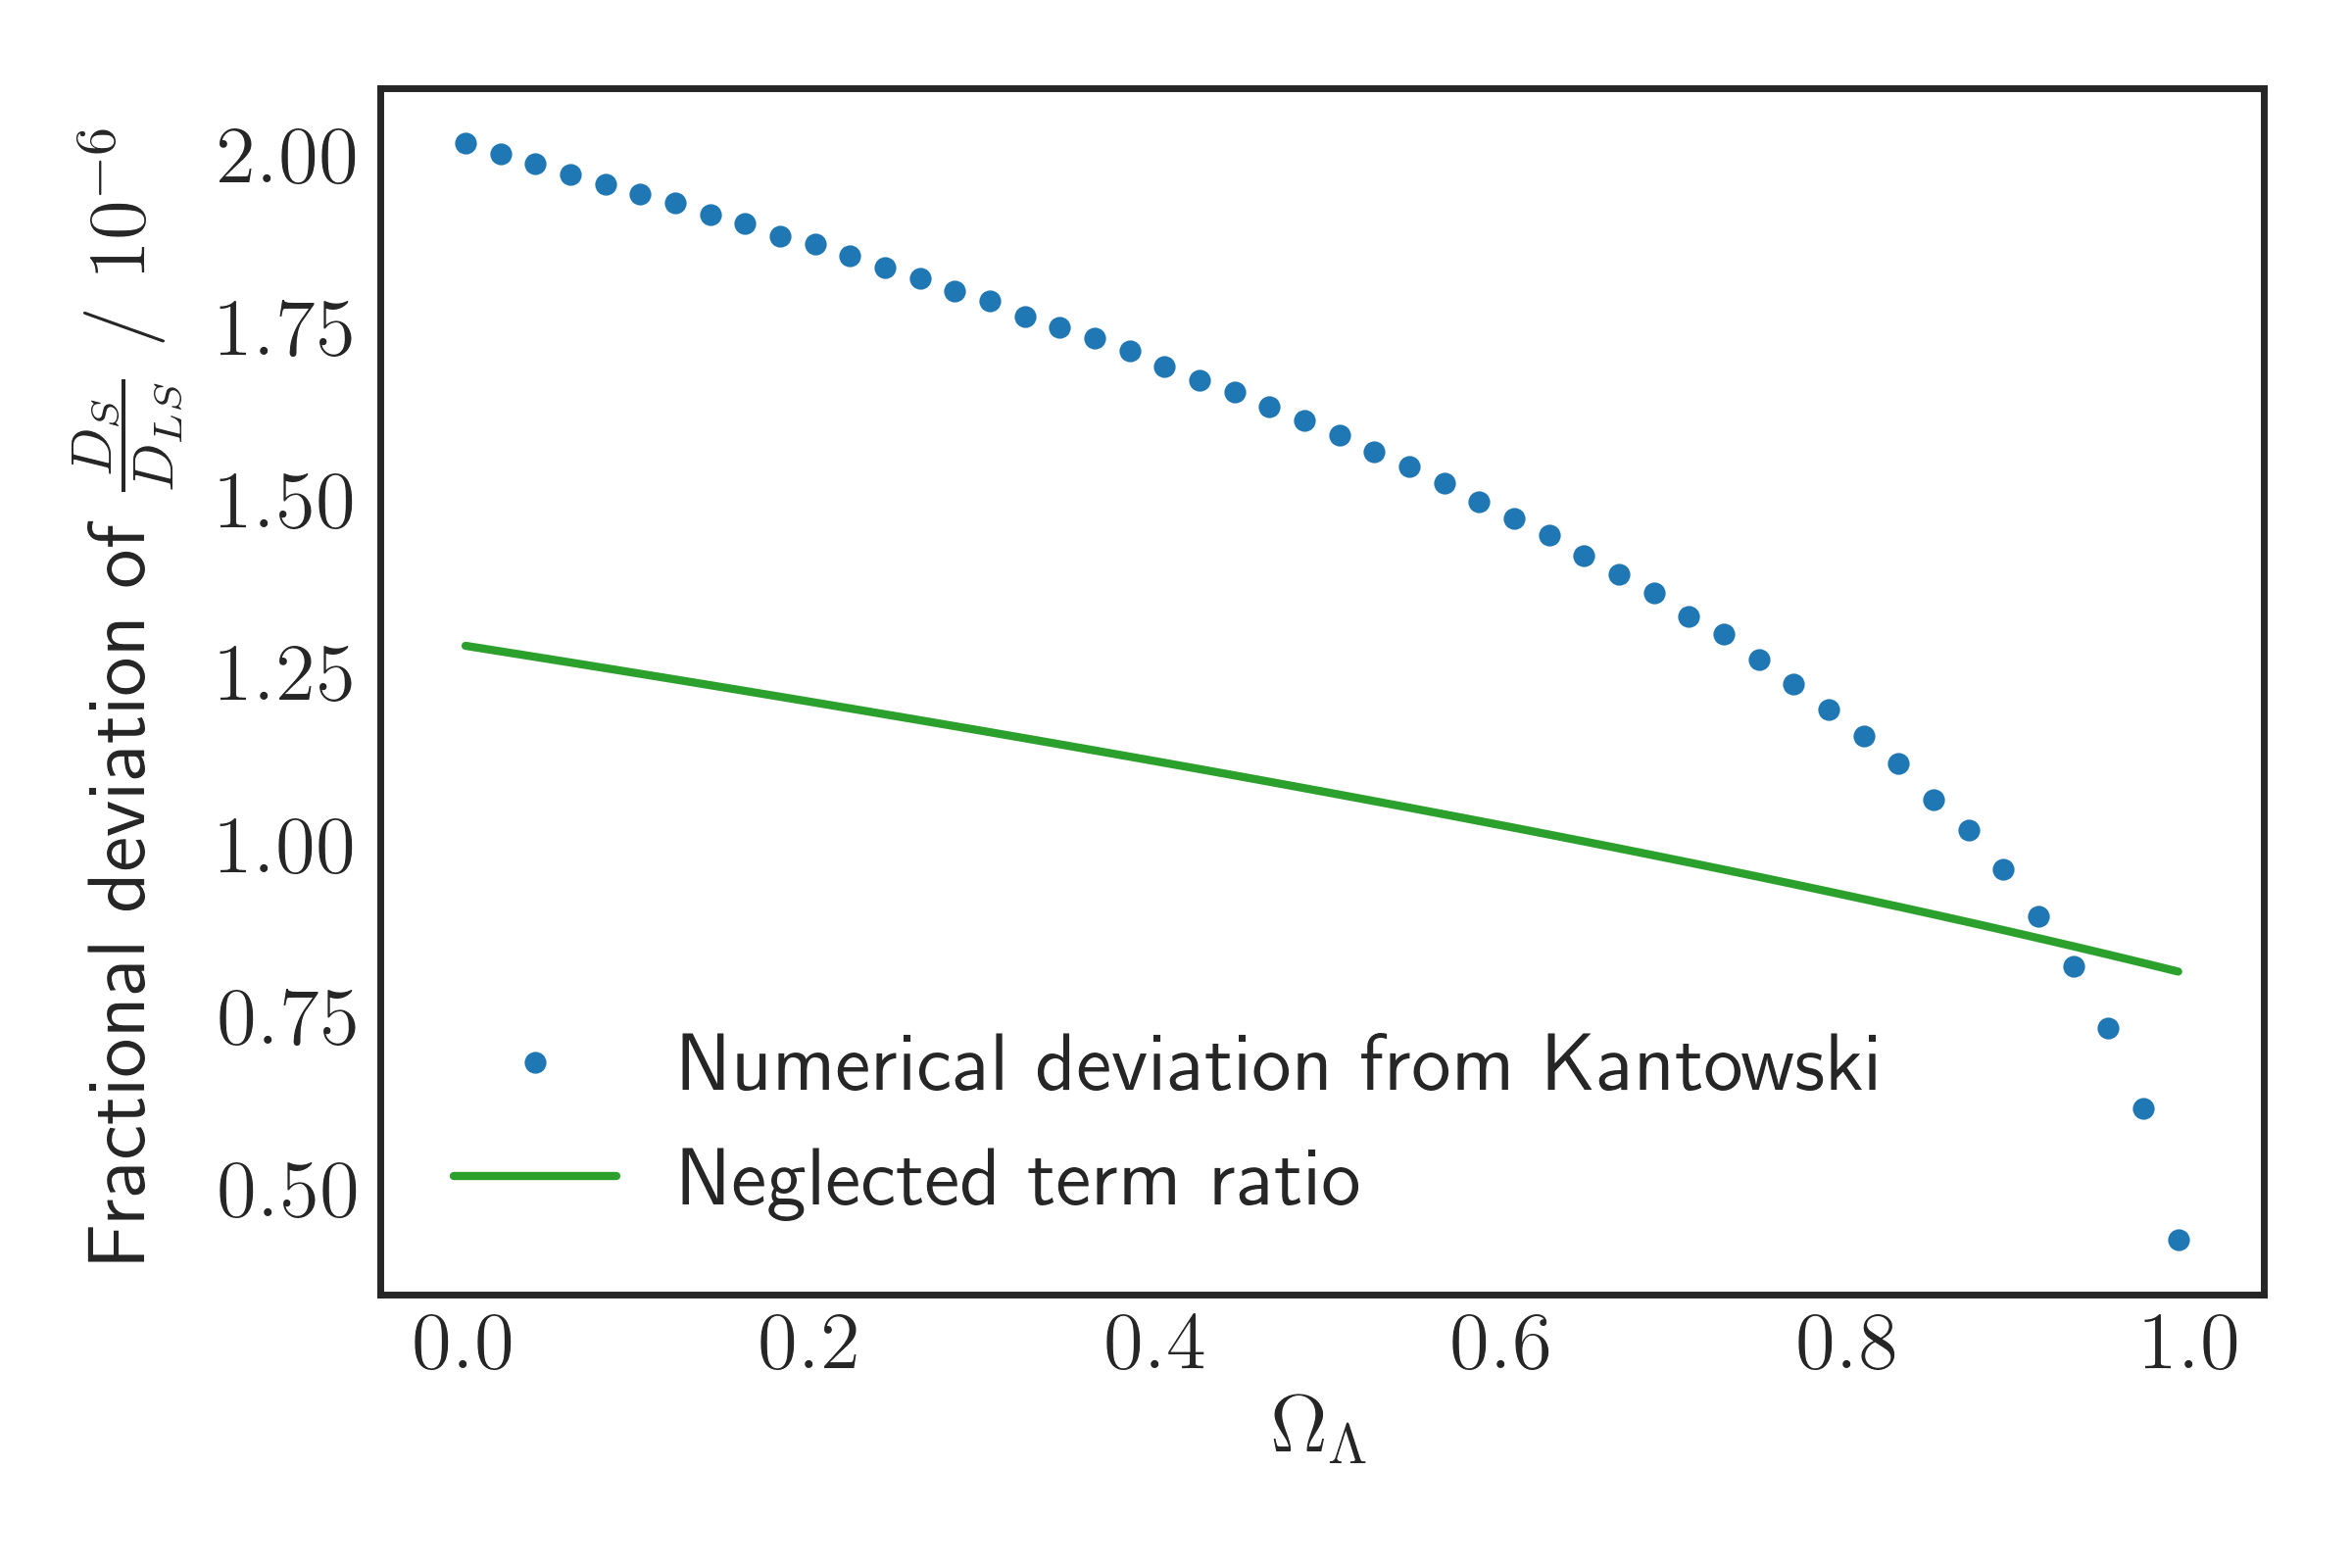
\includegraphics[height=0.5\linewidth]{images/flat-neglected.png}
  \caption{A plot of the absolute value of fractional numerical deviation from Kantowski's predictions, compared with the ratio of the higher order neglected term in Kantowski's calculation to his leading order term. They follow the same trend downwards, so it is a likely explanation that the difference is caused by the neglected higher order term.}
  \label{fig:flat-const-m-neglected}
\end{figure}

From the graph, we can see that even for the $\Lambda = 0$ case there is an offset between the numerical Swiss-cheese result and the FRW prediction. Qualitatively, this is due to the fact that conventional lensing analyis assumes a mass superimposed on the homogeneous background, and this mass has infinite range. However, in the Swiss-cheese model, the influence of the mass is limited, and bending stops once it leaves the Kottler hole. This is the main effect that Kantowski quantified in his paper \citet{kantowski2010gravitational}. This then begs the question of which model is a more accurate description of our physical universe, but this is not our primary concern. We are primarily concerned about whether $\Lambda$ has an influence on this effect. 

% At this point I wish to note that the applicability of this work of course hinges on the validity of the model we use, but this can be said of most scientific analysis. The Swiss-cheese model has been used in other areas in cosmology, not without success, as described in the introductory section of the previous chapter.  

There are a few different factors at play here. In discussing the results of this numerical integration, let us take a step back to look at the specific parts of ray-tracing that have a $\Lambda$-dependence. These are:
\begin{enumerate}
  \item The size of the hole. This is governed by \autoref{eq:junction-conditions-mass-volume}. In flat space, increasing $\Omega_{\Lambda}$ implies decreasing $\Omega_{m}$, which corresponds to the matter density of the universe. If we are to keep the mass constant, the hole size would have to increase as we increase $\Omega_{\Lambda}$. 
  \item The rate of expansion of the hole in static Kottler coordinates, given by \autoref{eq:hole-expansion-in-kottler-dR-dT}.  
  \item The Jacobian at the boundary, given by \autoref{eq:kottler-to-frw-transform-jacobian}.
\end{enumerate}

The first effect does not seem to be a truly direct $\Lambda$ effect, merely a side effect that in a flat universe, changing $\Omega_{\Lambda}$ must imply a change in matter density, but ultimately, it is the size of the hole that is the true determining factor in this effect. 

Therefore we look into keeping the hole size constant while varying $\Lambda$. The results for this are shown in \autoref{fig:flat-const-rh}, for the case of flat space. If the hole size is kept constant, then the mass will have to change with $\Omega_{\Lambda}$. In this case, the comoving size of the hole was fixed at $\SI{2.60}{\mega\parsec}$, which corresponds to a mass of $10^{13}M_{\odot}$ at $\Omega_{\Lambda} = 0$. The lens redshift was kept at $z_L = 0.5$ and the Einstein angle was set to be $1^{\prime\prime}$.

There is a difference between numerical results and Kantowski's predictions similar to the previous result that decreases with increasing $\Omega_{\Lambda}$. This was plotted in \autoref{fig:flat-const-rh-neglected} and indeed as we expect, the magnitude of the neglected higher-order term in his calculation follow the same general trend.

\begin{figure}
  \centering
  % \makebox[\linewidth][c]{%
  \begin{subfigure}{0.8\textwidth}
    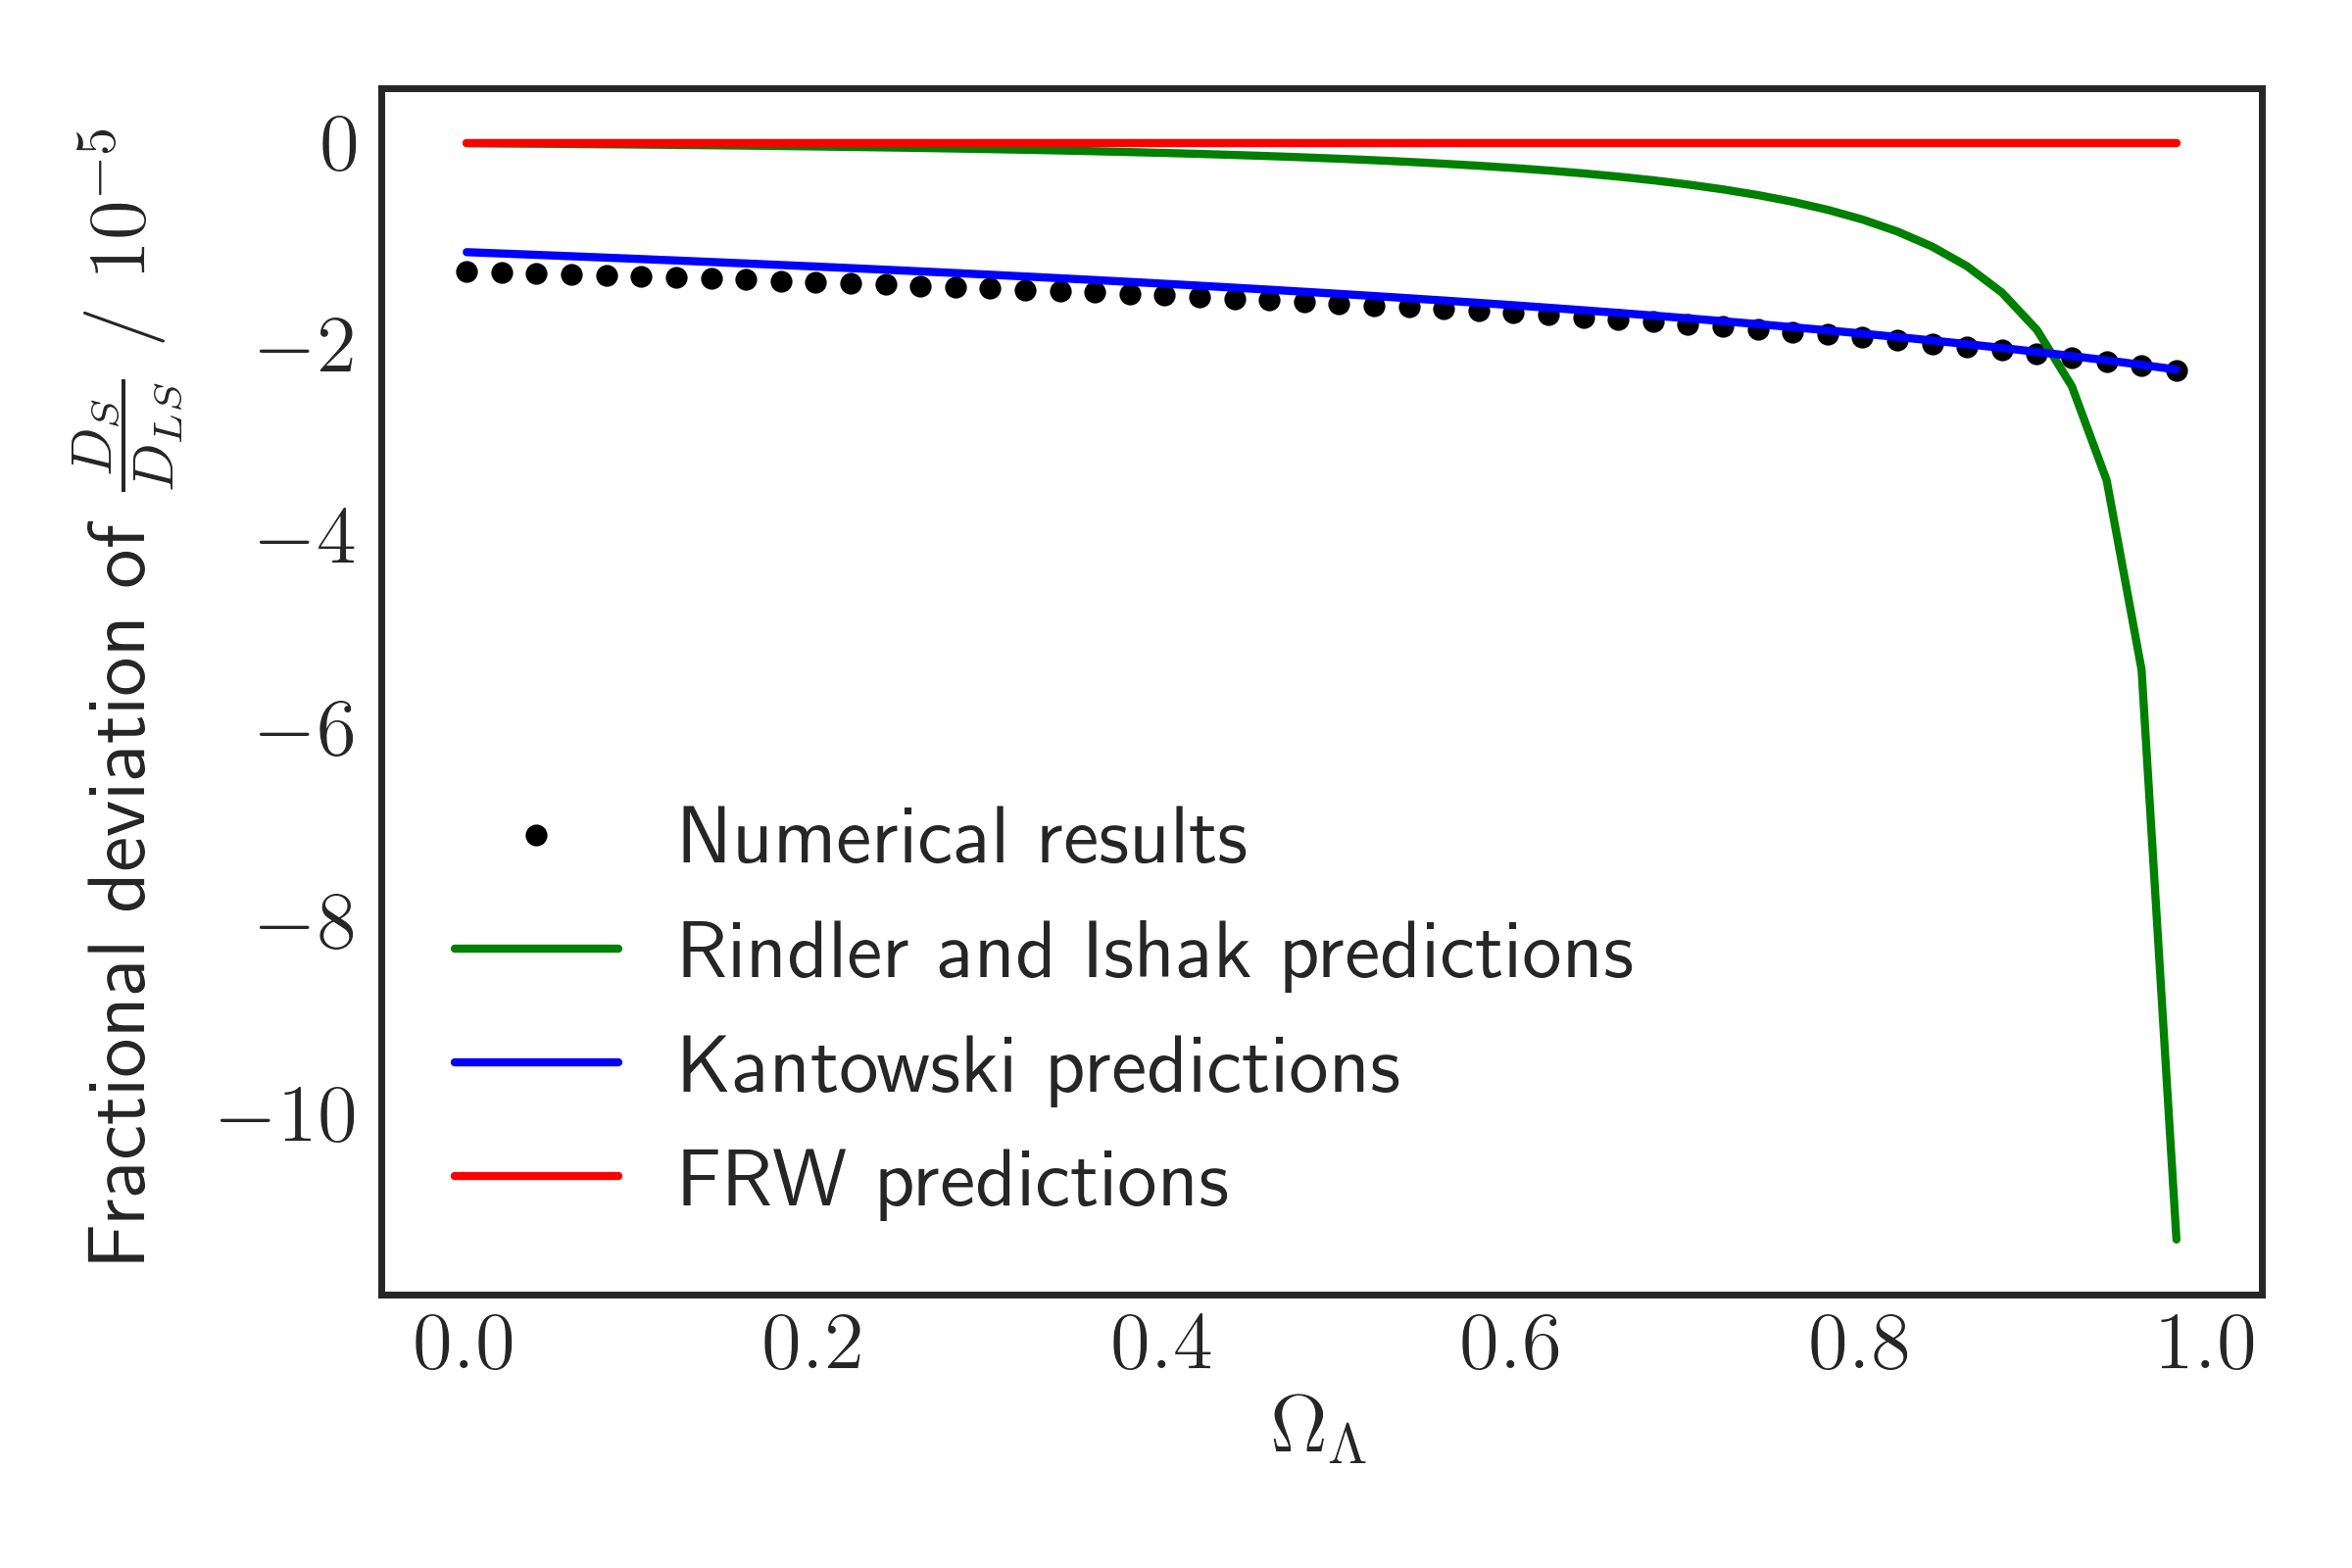
\includegraphics[width=\textwidth]{images/flat_const_rh.png}
    \caption{$\Omega_{\Lambda} = 0$ to $0.99$}
  \end{subfigure}%

  \begin{subfigure}{0.8\textwidth}
    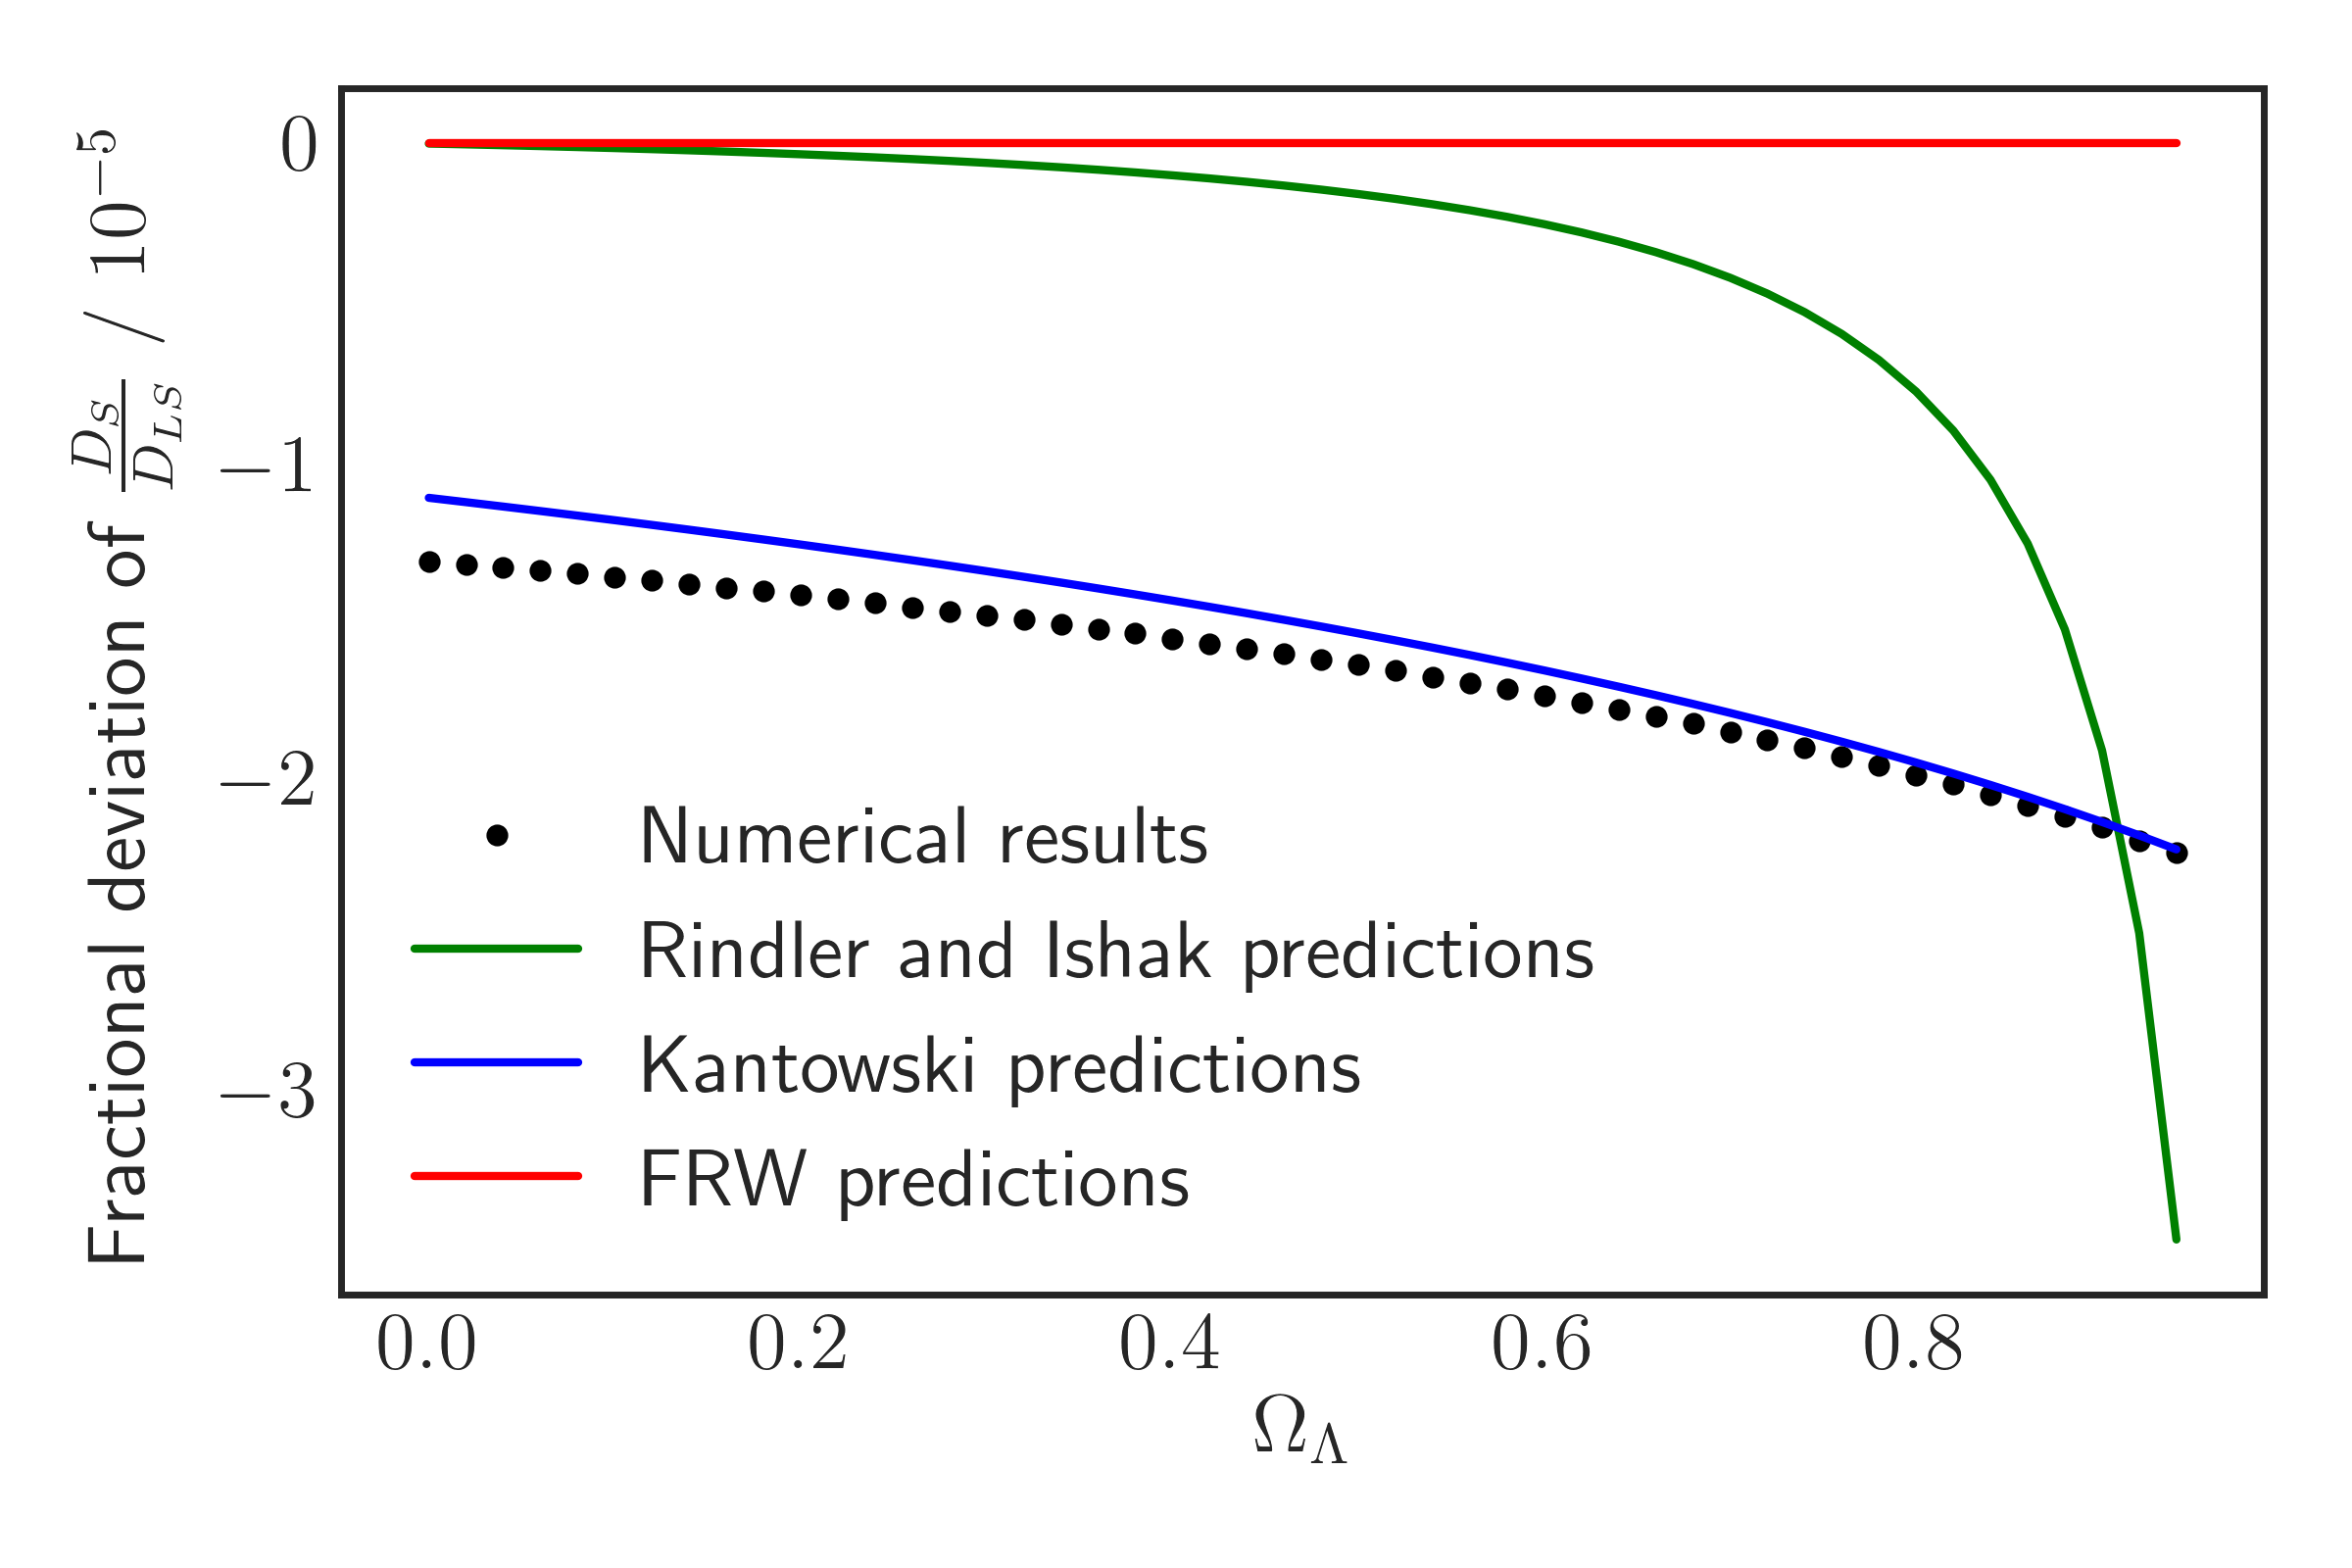
\includegraphics[width=\textwidth]{images/flat_const_rh2.png}
    \caption{$\Omega_{\Lambda} = 0$ to $0.95$}
  \end{subfigure}%
  % }%
  \caption{Results of the numerical simulation in flat space when $r_h$ is kept constant instead of $M$. The comoving size of the hole was fixed at $\SI{2.60}{\mega\parsec}$. This is the size such that at $\Omega_{\Lambda} = 0$, $M = 10^{13}M_{\odot}$. The left figure contains the full range from $\Omega_{\Lambda} = 0$ to $0.99$, whereas the right figure is the slightly zoomed in version after removing two of the rightmost points, to make the differences at lower $\Omega_{\Lambda}$ more apparent.}
  \label{fig:flat-const-rh}
\end{figure}


% \begin{figure}
% \centering
% \subcaptionbox[Short Subcaption]{%
%     $\Omega_{\Lambda} = 0$ to $0.99$%
%     \label{subfig:sublabel1}%
% }
% [%
%     0.8\textwidth % width of caption
% ]%
% {%
%     \includegraphics[width=0.8\textwidth]%
%     {images/flat_const_rh.png}%
% }%
% % \hspace{0.1\textwidth} % seperation
% \subcaptionbox[Short Subcaption]{%
%     $\Omega_{\Lambda} = 0$ to $0.95$%
% }
% [%
%     0.8\textwidth % width of caption
% ]%
% {%
%     \includegraphics[width=0.8\textwidth]%
%     {images/flat_const_rh2.png}%
% }%
% \caption[Short Caption]{Results of the numerical simulation in flat space when $r_h$ is kept constant instead of $M$. The comoving size of the hole was fixed at $\SI{2.60}{\mega\parsec}$. This is the size such that at $\Omega_{\Lambda} = 0$, $M = 10^{13}M_{\odot}$. The left figure contains the full range from $\Omega_{\Lambda} = 0$ to 0.99, whereas the right figure is the slightly zoomed in version after removing two of the rightmost points, to make the differences at lower $\Omega_{\Lambda}$ more apparent.}
% \label{fig:flat-const-rh}
% \end{figure}



\begin{figure}
  \centering
  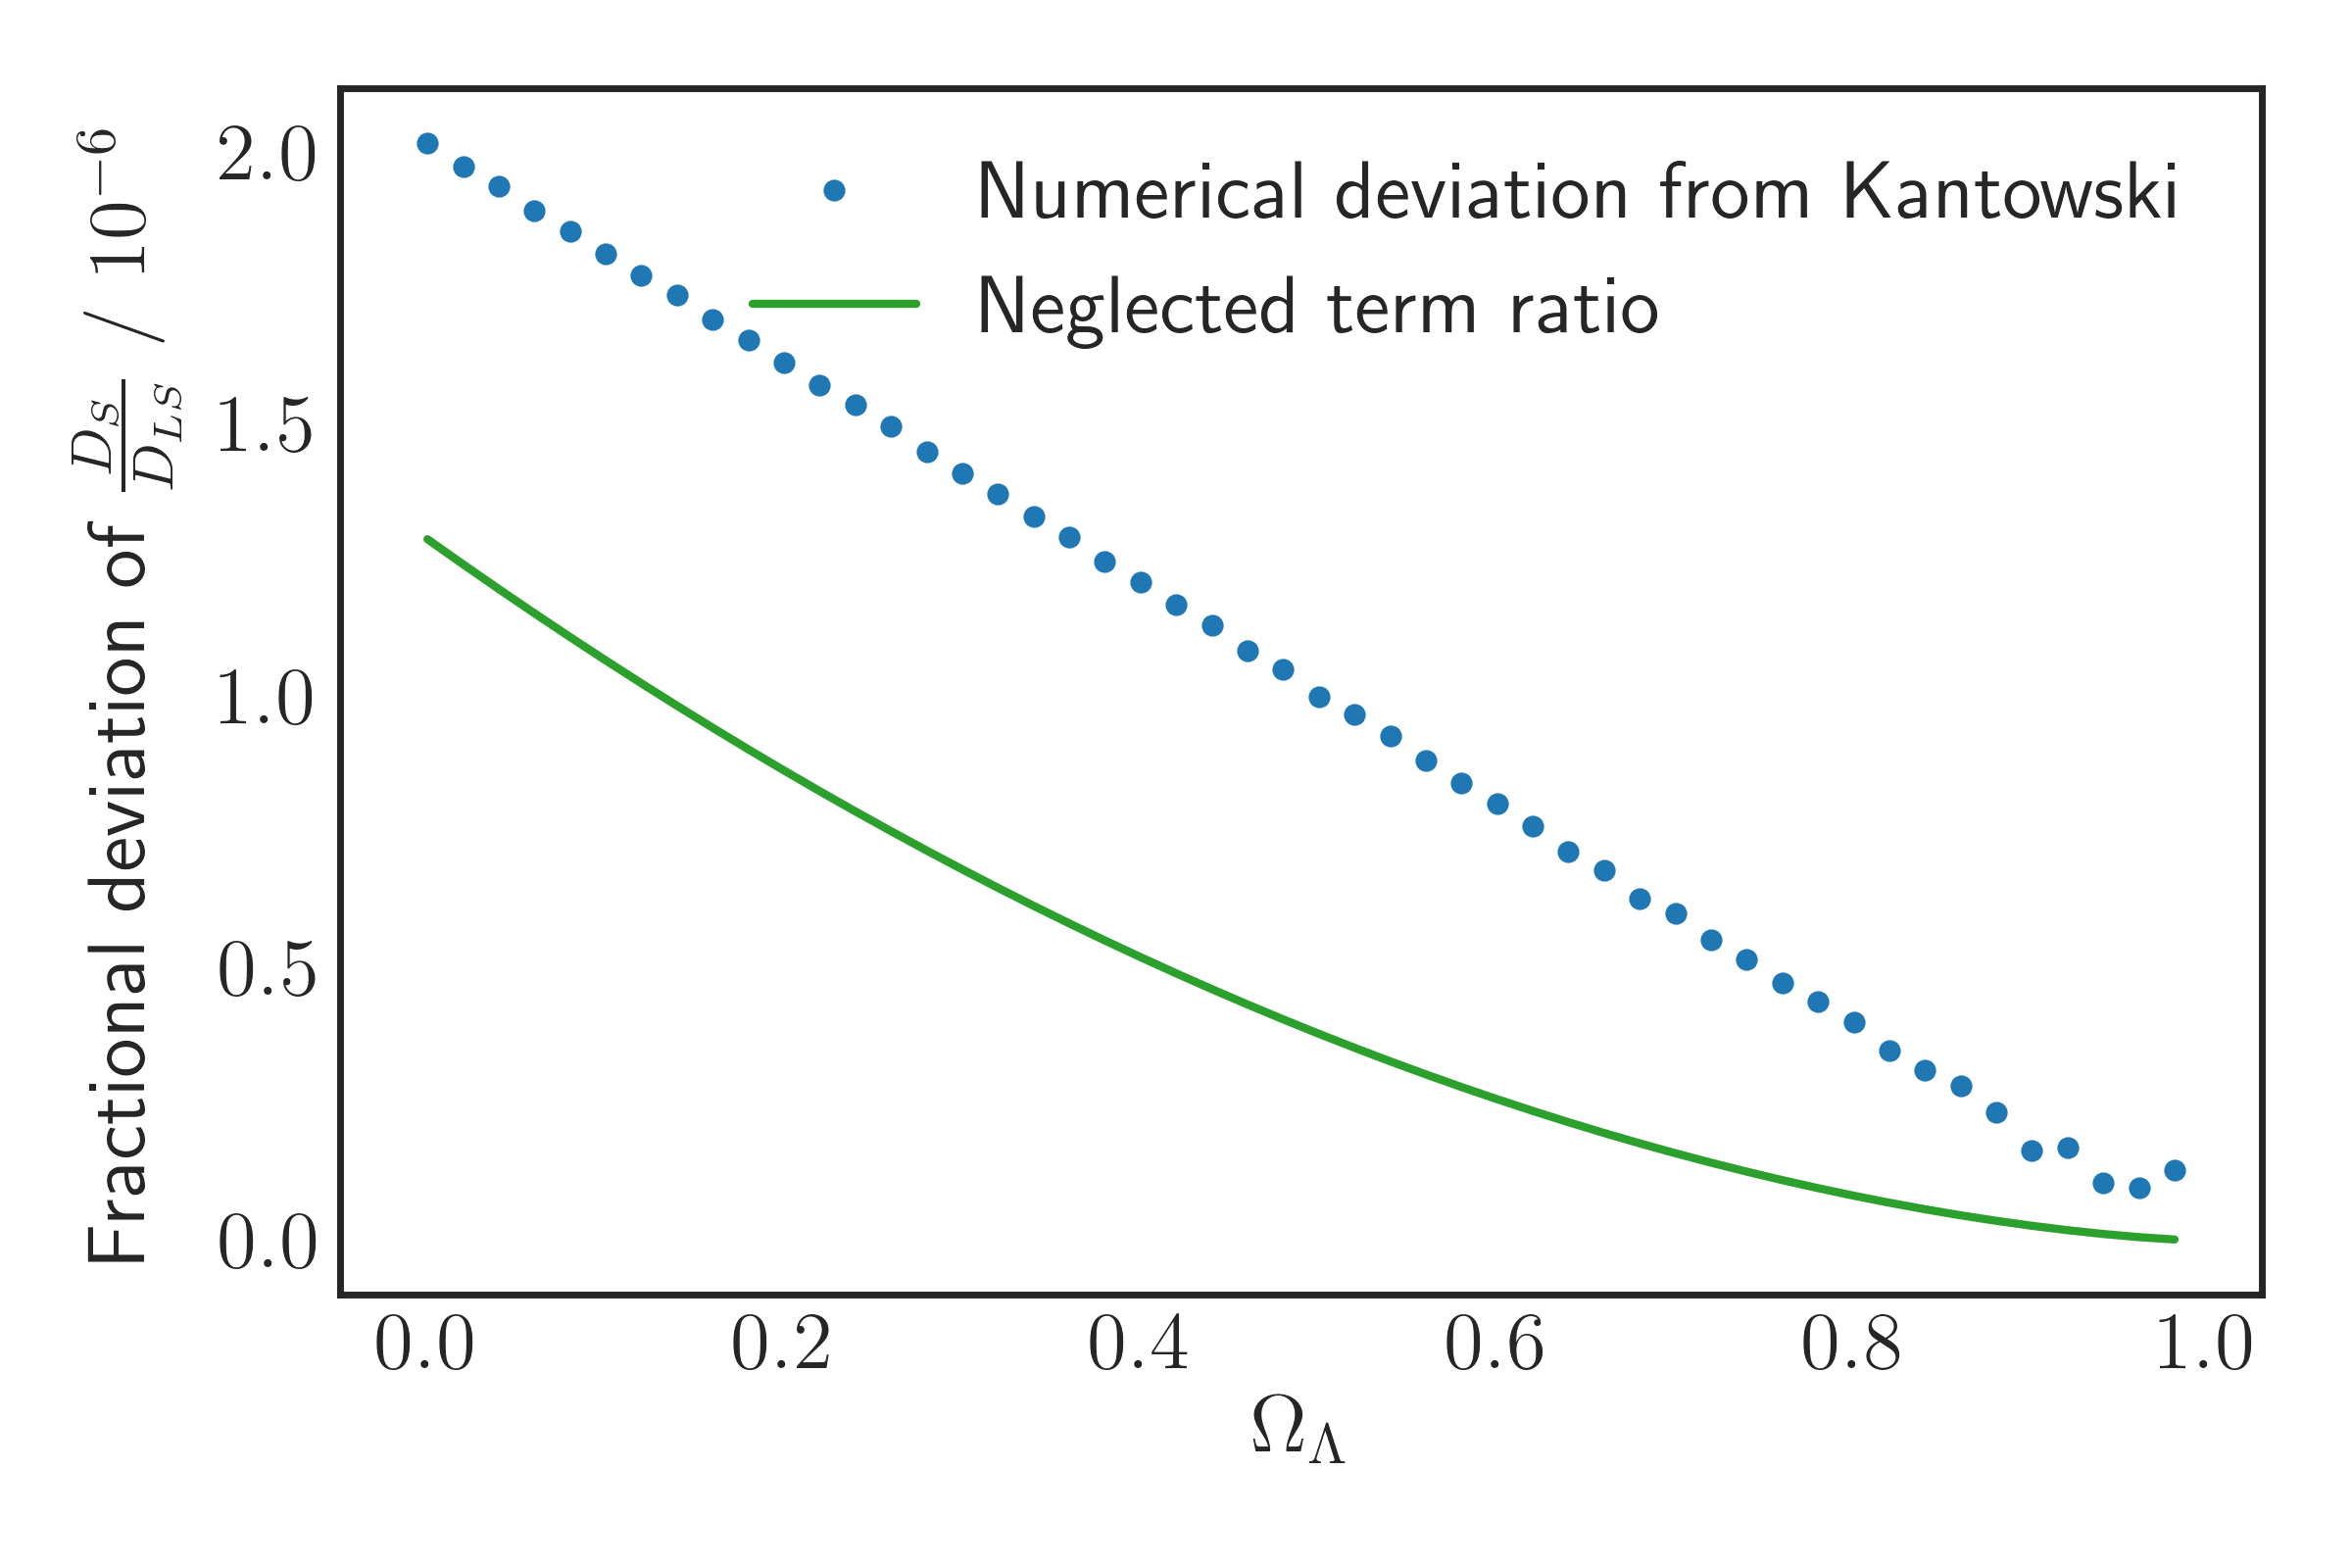
\includegraphics[height=0.5\linewidth]{images/flat-neglected_const_rh.png}
  \caption{A plot of the fractional deviation of numerical results from Kantowski's predictions, together with the ratio of the higher order term magnitude neglected in his calculations to his leading order term. }
  \label{fig:flat-const-rh-neglected}
\end{figure}

If we extend the integration for a universe with arbitrary curvature, then it is possible to fix both mass and $r_h$, but it would involve changing the curvature to compensate for the change in $\Lambda$. However, from the previous chapter, the curvature $k$ affects the rate of expansion of the Kottler hole and also enters into the Jacobian at the boundary as well, so intuitively one would expect $k$ to also have an effect on the bending angle in a Swiss-cheese model, though this effect has not been explored fully in literature (Kantowski's calculation \citet{kantowski2010gravitational} only applies for flat space). 

We have plotted the result of varying curvature to account for the change in $\Lambda$ in \autoref{fig:curved}. However, the results imply that the correction from curvature is even bigger than the $\Lambda$-effect, and hence it is unlikely to be useful. 

Unfortunately, there is no way to keep both curvature and matter density constant while varying $\Lambda$, so we cannot truly isolate the effect of $\Lambda$. Ultimately, to compensate for a change in $\Lambda$, one has to vary either matter density or curvature, or both. In a Swiss-cheese model, both factors are expected to affect the lensing observables to some extent. Given the limited literature on the effect of curvature on lensing in the Swiss-cheese model, and the much larger deviations resulting from curvature based on our numerical simulations (\autoref{fig:curved}), I would postulate that the variation of matter density has a smaller and better studied effect on lensing, and it is this we should vary such that the influence of $\Lambda$ becomes most apparent. Moreover, current cosmological observations \citep{ade2016planck,hinshaw2013nine,de2000flat} suggest quite convincingly that the Universe is spatially flat, and therefore looking at the case of $\Omega_k = 0$ is most appropriate. 

\begin{figure}
  \centering
  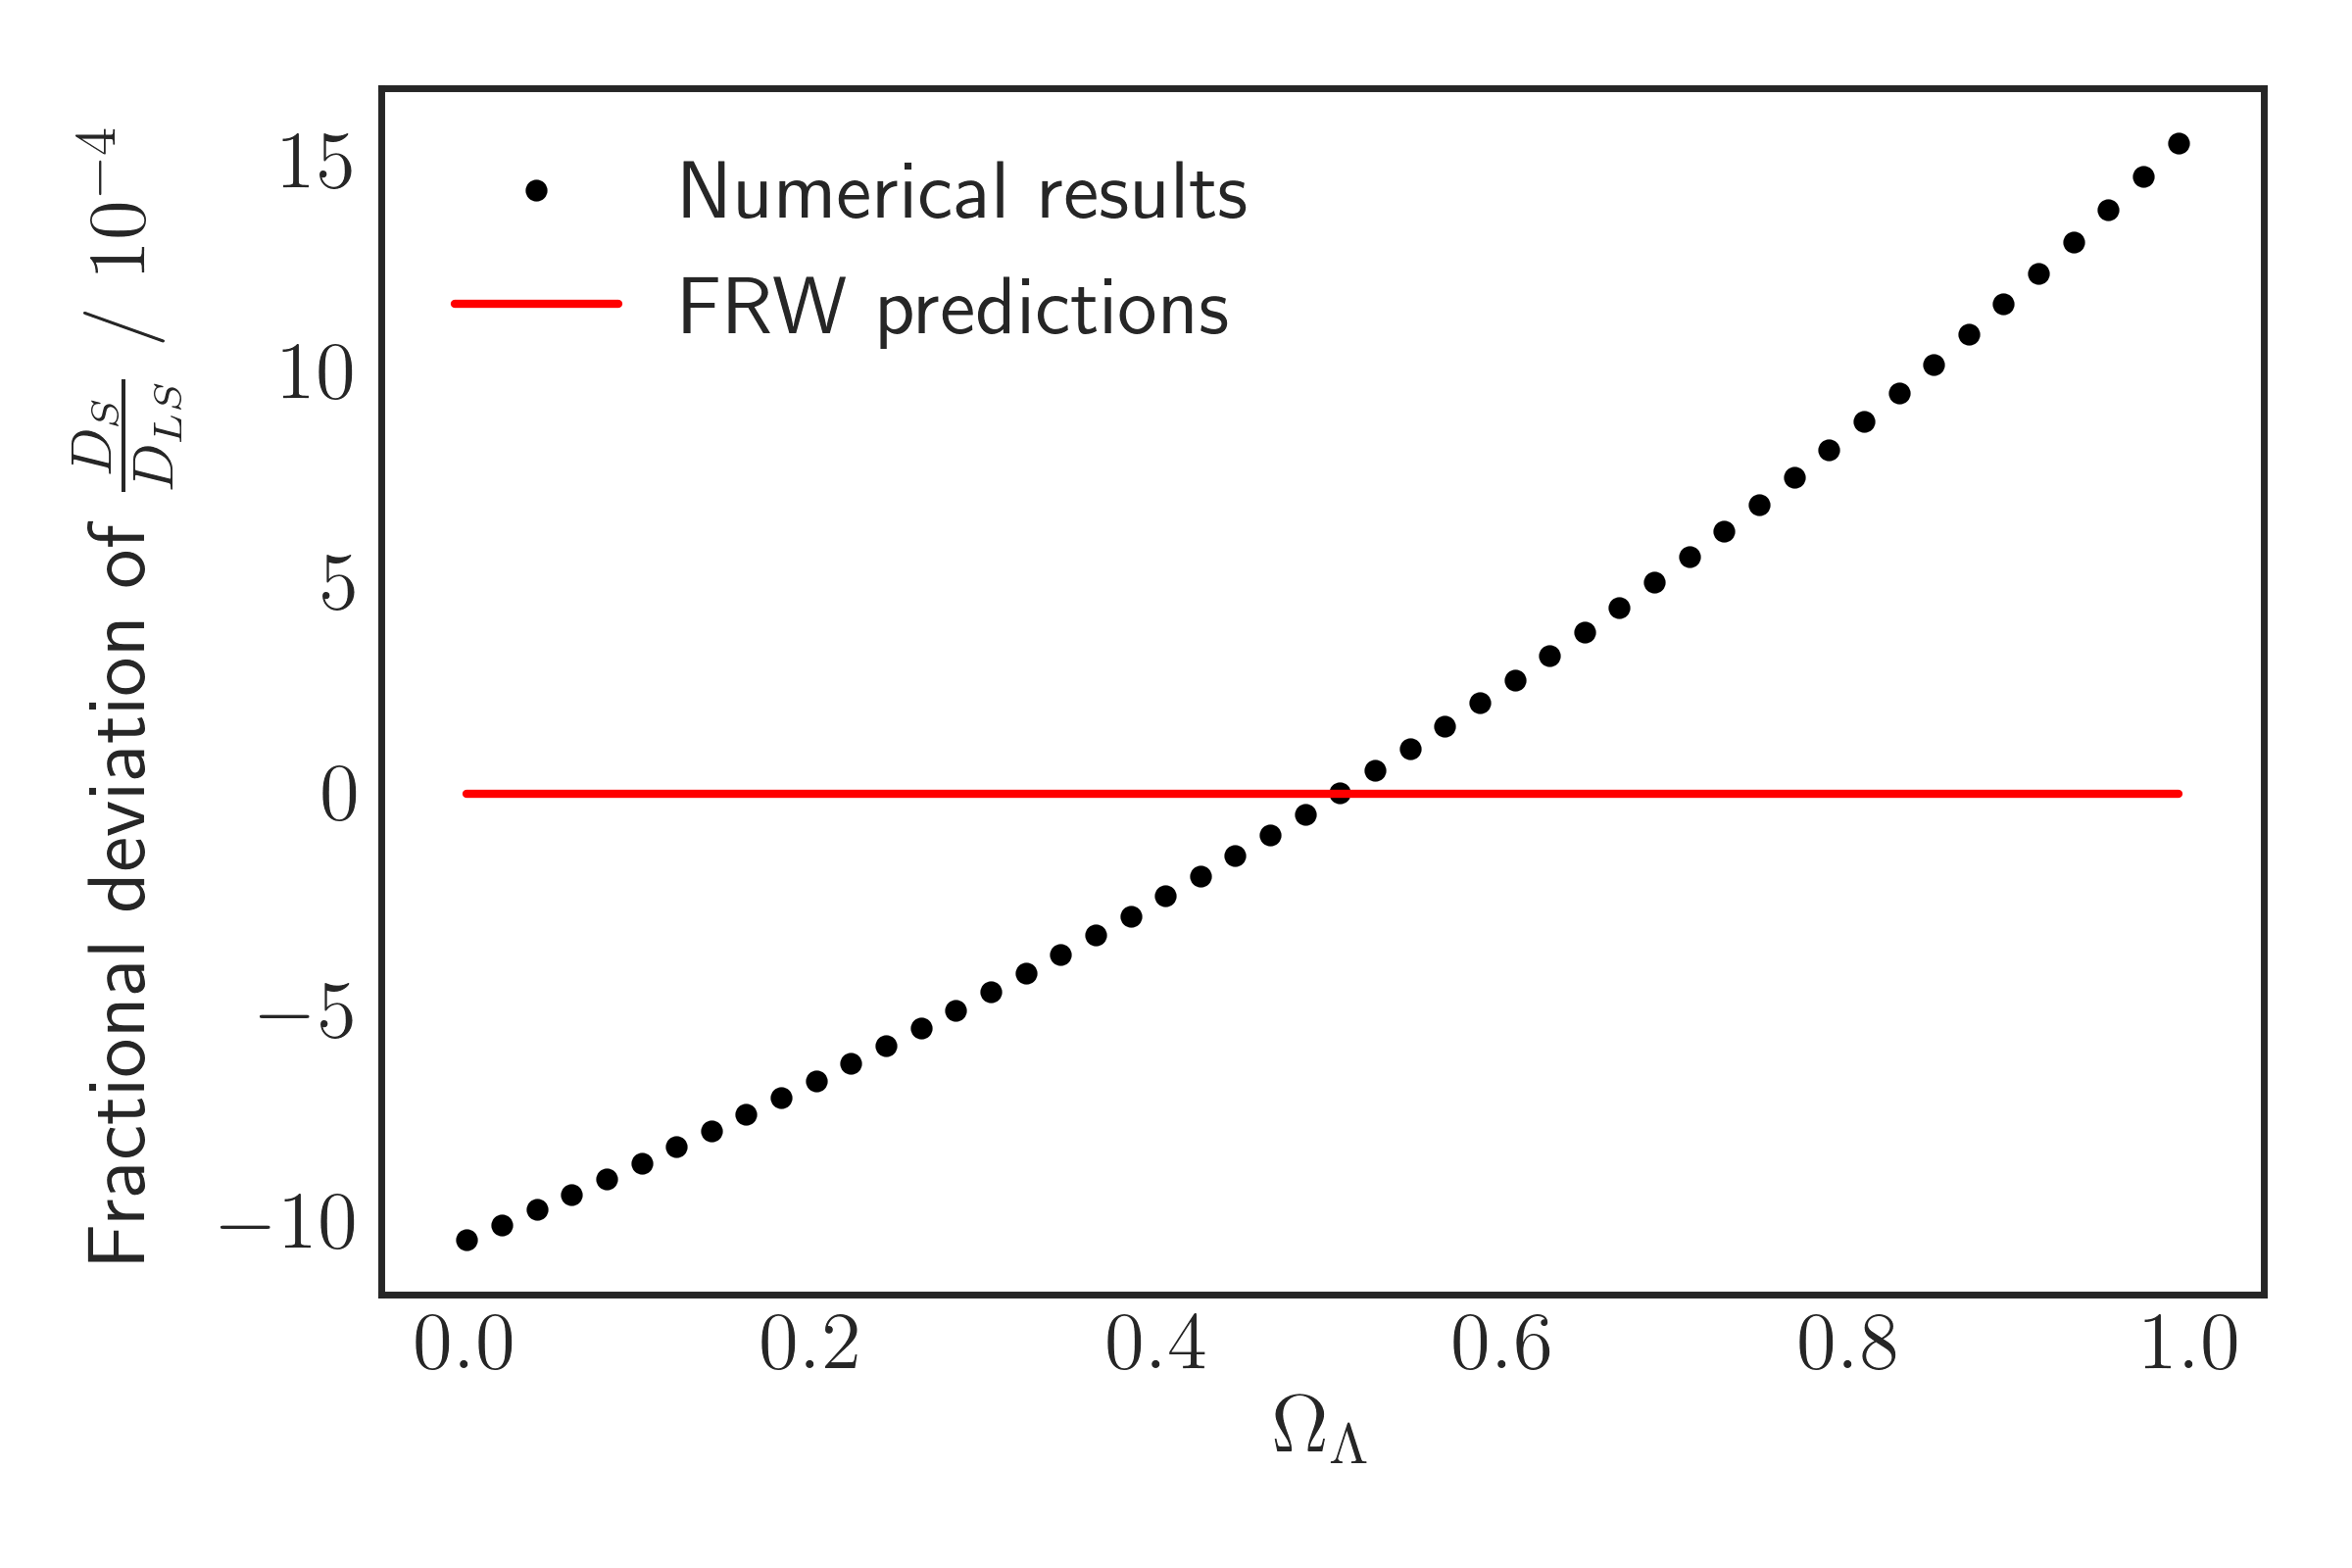
\includegraphics[height=0.5\linewidth]{images/curved.png}
  \caption{Plot of the results when $\Omega_{m}$ was kept constant at 0.5, $\Omega_{\Lambda} = 0$ to $0.99$ and $\Omega_k$ was used to compensate for the change in $\Omega_{\Lambda}$. The parameters used are $z = 0.5$, $M = 10^{13} M_{\odot}$. The numerical deviation is much bigger than the Rindler \& Ishak prediction and Kantowski prediction.}
  \label{fig:curved}
\end{figure}

Hence \autoref{fig:flat-const-rh} is the graph of most significance. From the graph we can see that while there is a clear trend when varying $\Lambda$, this is smaller than that in \autoref{fig:flat-const-m}, since the effect of different hole radius is eliminated. Similar to \autoref{fig:flat-const-m}, there is an offset even when $\Lambda = 0$, due to the truncation of bending at the hole boundary. 

Instead of comparing against the conventional FRW results, it is also instructive to compare the numerical results against the $\Lambda = 0$ point also obtained from numerical simulations, in a crude attempt to eliminate the effect at $\Lambda = 0$. These fractional deviations are even smaller than the deviations from the FRW result, at the order of $10^{-6}$. These are $10$ to $100$ times smaller than second order mass terms, which are routinely neglected. 

It was also pointed out by \citet{butcher2016no} that there is an unavoidable ambiguity when determining the distances $D_L$, $D_{LS}$, and $D_S$. In this work we have used \emph{unlensed} distances, that is, the distances were calculated as if the lens did not exist, when in reality the angular diameter distances are necessarily modified by the existence of the lens. According to Butcher's calculations, the fractional uncertainty arising from using unlensed distances is given by

\begin{equation}
  \frac{\delta D}{D} = \mathcal{O}\left (\frac{M}{\Lambda r^2} \right )
\end{equation}

For the parameters we are using, $z_L = 0.5$ and $M = 10^{13} M_{\odot}$ and $\Omega_{\Lambda} = 0.7$, we obtain a fractional uncertainty of about $10^{-9}$, which is much smaller than the magnitude that we are considering. 

% error estimation